We finally have all the main ingredients to generalize our line integral detour and discuss integration of $n$-forms over $n$-dimensional manifolds.

\newthought{We know from calculus one}, or our line integral examples, that the direction in which we traverse the interval, or a curve, can actually make a difference.
As it turns out, the sign of the integral of a differential $n$-form is only fixed after choosing an orientation of the manifold.
But what is an orientation?

If for a curve an orientation is simply a choice of a direction along it, so we can make sense of it in terms of a clockwise or a counter-clockwise motion, generalising the concept will require an extra abstraction step.
Not just that, you have seen already that in $\R^n$ there is a notion of standard orientation, but in other vector spaces we may need to make arbitrary choices.
For manifolds, the situation is much more complicated: for example, on a M\"obius strip\footnote{Cf. Example~\ref{ex:mobius}.} it is impossible to make any such choice, it is non-orientable.

\section{Orientation on vector spaces}
Let's proceed step by step by first revisiting some results from multivariable analysis. If you need a reference to review this material, you can refer to \cite[Chapter 6.2]{book:abrahammarsdenratiu} or \cite[Chapters 21.1-21.2]{book:tu}.

\begin{definition}
  Let $V$ be a one-dimensional vector space. Then $V\setminus\{0\}$ has two components.
  An \emph{orientation} of $V$ is a choice of one of these components, which one then labels as ``positive'' and ``negative''.
  A \emph{positive basis} of $V$ then is a choice of any non-zero vector belonging to the positive component, while a \emph{negative basis} of $V$ is a choice of any non-zero vector belonging to the negative component.
\end{definition}

\begin{example}
  The standard orientation of $\R$ is give by declaring that the positive numbers are the positive components of $\R\setminus\{0\}$.
  A common choice as positive basis for $\R$ is $\{e_1 \equiv 1\}$ while a negative basis could be $\{-e_1\}$.
\end{example}

If $V$ be a $n$-dimensional vector space, we know by Proposition~\ref{prop:dimLkV}, that $\Lambda^n(V)$ is a one-dimensional vector space.
Moreover, if $\{e_1,\ldots,e_n\}$ is a basis for $V$, then $e^1\wedge\cdots\wedge e^n$ is a basis for $\Lambda^n(V)$.

\begin{definition}
  Let $V$ be a $n$-dimensional vector space.
  An \emph{orientation} on $V$ is a choice of orientation\footnote{That is, we are talking about a representative from an equivalence class.} on the one-dimensional vector space $\Lambda^n(V)$.
  Therefore there are exactly two orientations: we say that a basis $\{e_1,\ldots,e_n\}$ of $V$ is \emph{positive} (or positively oriented) if $e^1\wedge\cdots\wedge e^n$ is a positive basis of $\Lambda^n(V)$ and \emph{negative} (or negatively oriented) otherwise.
\end{definition}

\begin{example}
  If $e_i$ is the standard $i$th basis vector in $\R^n$, the standard orientation of $\R^n$ is given by declaring that $e^1\wedge\cdots\wedge e^n$ is a positive basis of $\Lambda^n(\R^n)$ and thus that $\{e_1,\ldots,e_n\}$ is a positive basis of $\R^n$.
\end{example}

An automorphism $T:V\to V$ is called \emph{orientation-preserving} if it maps positively oriented bases to positively oriented bases (and \emph{orientation-reversing} otherwise).
Due to the way different bases are transformed by $n$-forms, this is equivalent to say that $\det T > 0$.

% indeed, let $\{v_1, \ldots, v_n\}$ be a positively oriented basis and $w_i = T v_i$, then
% \begin{align}
%   v^1\wedge\cdots\wedge v^n (w_1, \ldots, w_n) &= v^1\wedge\cdots\wedge v^n (Tv_1, \ldots, Tv_n) \\
%   &= \det(T)\; v^1\wedge\cdots\wedge v^n (v_1, \ldots, v_n) \\
%   &= \det(T).
% \end{align}

In fact, the orientation is completely characterized by the action of $n$-forms on the bases, as the following lemma shows.

\begin{lemma}\label{lemma:orient}
  Let $V$ be a $n$-dimensional vector space and let $ \omega\in\Lambda^n(V)$ be nowhere vanishing.
  Then, all bases $\{v_1, \ldots, v_n\}$ for which $\omega(v_1,\ldots, v_n) > 0$ give the same\footnote{Not necessarily the positive orientation!} orientation for $V$.
\end{lemma}
% \begin{proof}
%   Let $\{v_1, \ldots, v_n\}$ and $\{w_1, \ldots, w_n\}$ denote two different bases for $V$, then there exists a linear isomorphism $\varphi$ such that $v = \varphi\, w$, that is $v_i = \varphi_{i}^j w_j$.
%   By definition and by multilinearity we then have
%   \begin{equation}\label{eq:posorie}
%     0 < \omega(v_1,\ldots v_n) = \omega(\varphi\, w_1,\ldots \varphi\, w_n) = \det(\varphi)\omega(w_1,\ldots w_n),
%   \end{equation} that is the positivity of $\omega$ on the bases characterize the set of bases.
% \end{proof}

\begin{exercise}
  Let $V$ be a $n$-dimensional vector space, prove that two nonzero $n$-forms on $V$ determine the same orientation if and only if each is a positive multiple of the other.
\end{exercise}

This allows to define an eqivalence relation between orientations in terms of the nonzero elements in $\Lambda^n(V)$. We call these nonzero elements \emph{volume elements}.

Two volume elements $\omega_1, \omega_2$ are equivalent if there exists $c > 0$ such that $\omega_1 = c\, \omega_2$.
Then, the previous exercise implies that the classes of equivalence $[\omega]$ of volume elments on $V$ uniquely determine orientations on $V$.

\begin{remark}
  Of course, if $V$ is a vector space, then an orientation on $V$ canonically determines an orientation on the dual space $V^*$ by declaring that the basis dual to a positive basis is itself positive.
\end{remark}

We now need to extend all this to manifolds.

\section{Orientation on manifolds}
Tangent and cotangent spaces are vector spaces, so what we discussed in the previous section directly apply (as usual).
Moreover, we can bundle up over our manifold into a vector bundle.
Differential $n$-forms, then, seem a reasonable concept to define a notion of orientation for a manifold, at least if we think about their pointwise meaning of assigning an orientation to each fiber of $TM$.

\begin{definition}
  A \emph{volume form} on a $n$-dimensional smooth manifold $M$ is a $n$-form $\omega\in\Omega^n(M)$ such that $\omega(p) \neq 0$ for all $p\in M$.
  We say that $M$ is \emph{orientable} if there exists a volume form on $M$.
\end{definition}

\begin{example}
  According to this defitinion $\R^3$ has the standard volume form $\omega = dx \wedge dy \wedge dz$.
\end{example}

Of course, one does need to make sure that locally we can make sense of this concept of orientation for it to even make sense as a definition.
  By Lemma~\ref{lemma:orient} each chart $(U, \varphi)$ in the atlas determines an orientation at each point of its domain, which will be positive if $\det(d\varphi)>0$ and negative otherwise.
  This procedure can be repeated for each chart in an atlas for $M$.
  Thus, in order to get a globally consistent ordering, we need to worry about the overlaps between charts.

\begin{proposition}\label{prop:orientable}
  Let $M$ be a smooth, connected\marginnote{If it is not connected, then we need to deal with each connected component separately.} $n$-manifold.
  Then the following are equivalent:
  \begin{enumerate}
    \item $M$ is orientable;
    \item there exists $\omega\in\Omega^n(M)$ such that every other $\eta\in\Omega^n(M)$ may be written as $\eta = f\,\omega$ for some $f\in C^\infty(M)$;
    \item $M$ has an atlas $\{(U_i, \phi_i)\}$ such that the Jacobian determinant of the transition maps is positive\footnote{That is, $\det(D\varphi_{ij}) > 0$ for all the transition maps $\varphi_{ij} := \varphi_i\circ\varphi_j^{-1}$, and therefore all the charts have the same orientation.}. Such an atlas is said to be \emph{oriented}.
  \end{enumerate}
\end{proposition}
\begin{proof}
  \textbf{Part I: 1. $\Leftrightarrow$ 2.}
  Assume $M$ orientable with a volume form $\omega$ and let $\eta\in\Omega^n(M)$ be any other differential $n$-form.
  Since every fiber of $\Lambda^n M$ is one-dimensional, we can directly define $f:M \to \R$ pointwise via the equation
  \[
    \eta_p = f(p)\,\omega_p.
  \]
  We need to show that $f\in C^\infty(M)$.
  Locally, for some chart with coordinates $(x^i)$ on $M$, we have $\omega_p = w(p)\, dx^{i_1}\wedge\cdots\wedge dx^{i_n}$ and $\eta_p = \eta(p)\, dx^{i_1}\wedge\cdots\wedge dx^{i_n}$, where both coefficients are in  $C^\infty(M)$.
  Since $\omega(p) \neq 0$ for all $p\in M$, $f(p) = \eta(p)/\omega(p)$ is a smooth function.

  Conversely, if $\omega$ is a basis for $\Omega^n$, then it must be nonvanishing for all $p\in M$ since each fiber is one-dimensional.
  \medskip

  \textbf{Part II: 1. $\Leftrightarrow$ 3.}
  Assume $M$ is orientable witha volume form $\omega$.
  By eventually restricting the domains, let the atlas $\cA = \{(U_i, \varphi_i)\}$ be such that $\varphi_i(U_i) \subset \R^n$ is connected.
  Denote $\omega_0 = dx^1 \wedge\cdots\wedge dx^n$ the standard volume form on $\R^n$, then by the previous part of the proof, $(\varphi_i)_*\omega = f_i\,\omega_0$ for some smooth function $f_i \neq 0$.
  Without loss of generality\footnote{Is it clear why?} we can assume $f_i > 0$.
  % for the curious: this is because, modulo a reflection, we can always find a point x in the domain \phi_i(U_i) of f_i such that f_i(x) > 0. Since f_i must be nonnegative and is continuous on its connected domain, the function cannot change sign, that is, it must be > 0.

  Let $\varphi_k$ and $\varphi_l$ be two different charts in $\cA$ with overlapping domains (otherwise there is nothing to check).
   Define the transition map $\sigma_{kl} := \varphi_k\circ\varphi_l^{-1}$.
  \begin{align}
    (\sigma_{kl})_* dx^1\wedge\cdots\wedge dx^n &= (\varphi_k)_* \circ (\varphi_l^{-1})_* dx^1\wedge \cdots\wedge dx^n \\
                                         &= \frac{f_k}{f_l \circ \sigma_{lk}} dx^1\wedge \cdots\wedge dx^n. 
  \end{align}
  Thus, by Proposition~\ref{prop:wedgeToJDet}, we get
  \begin{equation}\label{form:cov}
    \det(D\sigma_{lk}) = \frac{f_k}{f_l \circ \sigma_{lk}} > 0.
  \end{equation}

  For the converse, let $\rho_i$ denote a partition of unity subordinate to the oriented atlas $\{(U_i, \varphi_i)\}$.
  Define
  \begin{equation}
    \omega_i := \varphi_i^* dx^1\wedge\cdots\wedge dx^n \in \Omega^n(U_i)
    , \qquad
    \widetilde \omega_i(p) := \begin{cases}
      \rho_i(p)\omega_i(p) & \mbox{if } p\in U_i \\
      0 & \mbox{otherwise}
    \end{cases}.
  \end{equation}
  Since $\supp(\rho_i) \subset U_i$, we have $\widetilde\omega_i\in\Omega^n(M)$.
  Let $\omega := \sum_i \widetilde \omega_i$. This sum is finite in a neigbourhood of each point so, in particular, $\omega \in \Omega^n(M)$. We need to show that it is a volume form on $M$.
  On nonempty overlaps $U_k \cap U_l \neq \emptyset$ of charts we have
  \begin{align}
    \omega_l &= \varphi_l^*\, dx^1\wedge\cdots\wedge dx^n = \varphi_k^* \sigma_{lk}^*\, dx^1 \wedge\cdots\wedge dx^n \\
             &= (\det(D\sigma_{lk})\circ \varphi_k)\circ \varphi^*_k\, dx^1\wedge\cdots\wedge dx^n \\
             &= (\det(D\sigma_{lk})\circ \varphi_k)\, \omega_k =: \alpha_{lk} \omega_k
  \end{align}
  where $\alpha_{lk}\in C^{\infty}(U_k\cap U_l)$, $a_{lk} > 0$ and there is no implied sum\footnote{All indices are low indices.}.
  Since the covering $\{U_i\}$ is locally finite\footnote{See Theorem~\ref{thm:partitionof1}.}, a point $p\in M$ belongs only to a finite number of open sets, let's call them $U_{i_0}, U_{i_1}, \ldots, U_{i_N}$. That is,
  \begin{equation}
  \omega(p) = \sum_{k=1}^N \omega_{i_k}(p) = \left( 1 + \sum_{k = 1}^N a_{i_k i_0} \right) \omega_{i_0}(p) \neq 0
  \end{equation}
  since $\omega_{i_0}(p) \neq 0$ and $a_{i_k i_0} > 0$.
  That is, for all $p\in M$ we have that $\omega(p) \neq 0$.
  \end{proof}


\begin{definition}
  A manifold $M$ with an oriented atlas is called \emph{oriented manifold}.
  If an orientation exists, we call \emph{orientation} the equivalence class of atlases with the same orientation.
  Otherwise we say that the manifold is \emph{non-orientable}.
\end{definition}

A consequence of Lemma~\ref{lemma:orient} and the first part of Proposition~\ref{prop:orientable} is that if a connected manifold is orientable, then there are exactly two different orientations.

\begin{definition}
  Let $M$ be an oriented smooth manifold.
  If $(U,\varphi)$ is a chart with local coordinates $(x^i)$ such that, in the coordinate representation, the volume form $\omega = \omega(x) dx^1\wedge\cdots\wedge dx^n$ with $\omega(x) > 0$, then we say that the chart $\varphi$ is \emph{positively oriented} with respect to $\omega$, otherwise we say that it is \emph{negatively oriented}.
  Similarly, if $M$ is connected and the charts for the oriented manifold are positively (resp. negatively) oriented, we say that the manifold is positively (resp. negatively) oriented.
\end{definition}
%
% \begin{theorem}
  %   Let $M$ be a $n$-dimensional smooth manifold.
%   A nowhere-vanishing $n$-form $\omega\in\Omega^n(M)$ uniquely determines an orientation.
%   For this reason, nowhere vanishing $n$-forms on a smooth $n$-manifold are called \emph{volume forms}.
% \end{theorem}
% \begin{proof}
%   Let $\varphi$ and $\psi$ be two different charts with overlapping domains (otherwise there is nothing to check) and with local coordinates $(x^i)$ and $(y^i)$ respectively.
%   Define the transition map $\sigma := \psi\circ\varphi^{-1}$, so that $(y^1,\ldots,y^n) = \sigma(x)$.
%   Since $d y^j = (D\sigma)_i^j dx^i$, we have that locally,
%   \marginnote[3.5em]{$\leftarrow\; x = \sigma^{-1}(y)$}
%   \begin{align}
%     \omega &= \widetilde \omega(y) dy^1\wedge\cdots\wedge dy^n \\
%     &= (\widetilde\omega \circ \sigma)(x) (D\sigma|_x)^1_{j_1}\cdots (D\sigma|_x)^n_{j_n} dx^{j_1}\wedge\cdots\wedge dx^{j_n} \\
%     &= (\widetilde\omega \circ \sigma)(x) \det(D\sigma|_x) dx^{1}\wedge\cdots\wedge dx^{n} \\
%     &= \sigma^*(\widetilde \omega(y) dy^1\wedge\cdots\wedge dy^n) \\
%     &= \omega(x) dx^{1}\wedge\cdots\wedge dx^{n},
%   \end{align}
%   where we used Proposition~\ref{prop:wedgeToJDet} and 
%   Theorem~\ref{thm:pullbacksdifferentialforms}.
%   Thus,
%   \begin{equation}\label{form:cov}
%     \omega(x) = (\widetilde\omega \circ \sigma)(x) \det(D\sigma|_x),
%   \end{equation}
%   and it has the same sign of $\widetilde\omega(y)$ if and only if $\det(D\sigma|_x) > 0$.
% \end{proof}
% 

\begin{example}\label{exe:orientsphere}
  Let $M = \bS^1\subset \R^2$.
  This is an orientable manifold and we can find an orientation using the stereographic projections from Exercise~\ref{ex:stereo}.
  Let $U_1 = \bS^1\setminus\{N\}$ and $U_2 = \bS^1\setminus\{S\}$, with the associated diffeomorphisms
  \begin{equation}
    \varphi_1(p) = \frac{2p^1}{1-p^2}
    \quad\mbox{and}\quad
    \varphi_2(p) = \frac{2p^1}{1+p^2}.
  \end{equation}
  Let's pick a pointwise orientation by choosing as basis $X_p\in T_pM$ given by\footnote{We are not making up anything, if you look carefully this is just $X_p = \partial_\theta$.} $X_p = -p^2 \frac{\partial}{\partial p^1} + p^1 \frac{\partial}{\partial p^2}$.
  Then, on $U_1$,
  \begin{align}
    (\varphi_1)_*(X) &= (d\varphi_1)_p(X) \\
    &= \left(\begin{smallmatrix}
      \frac{2}{1-p^2} & \frac{2p^1}{(1-p^2)^2}
    \end{smallmatrix}\right)
    \left(\begin{smallmatrix}
      -p^2 \\ p^1
    \end{smallmatrix}\right) \frac{\partial}{\partial x}\Big|_{\varphi_1(p)}\\
    &= \frac{2}{1-p^2} \frac{\partial}{\partial x}\Big|_{\varphi_1(p)},
  \end{align}
  and $\frac{2}{1-p^2}>0$.
  If we perform the same computation on $U_2$, however, we obtain $(\varphi_2)_*(X) = -\frac{2}{1+p^2}\frac{\partial}{\partial x}\Big|_{\varphi_2(p)}$, with the negative coefficient $-\frac{2}{1+p^2} < 0$, corresponding to the opposite orientation on $U_2$.
  Of course, in this case, not all is lost: by choosing $\widetilde\varphi_2(p) = \varphi_2(-p^1, p^2)$ we obtain $(\widetilde\varphi_2)_*(X) = \frac{2}{1+p^2} \frac{\partial}{\partial x}\Big|_{\widetilde\varphi_2(p)}$ with the positive coefficient $\frac{2}{1+p^2} > 0$, which shows that $X_p$ defines an orientation on the whole $\bS^1$.
\end{example}

\begin{exercise}
  Check that the Jacobian determinant $\det(D(\varphi_2\circ \varphi_1^{-1}))$ of the transition chart from Exercise~\ref{exe:orientsphere} is negative, while $\det(D(\widetilde\varphi_2\circ \varphi_1^{-1}))$ is positive.
\end{exercise}

\begin{marginfigure}
  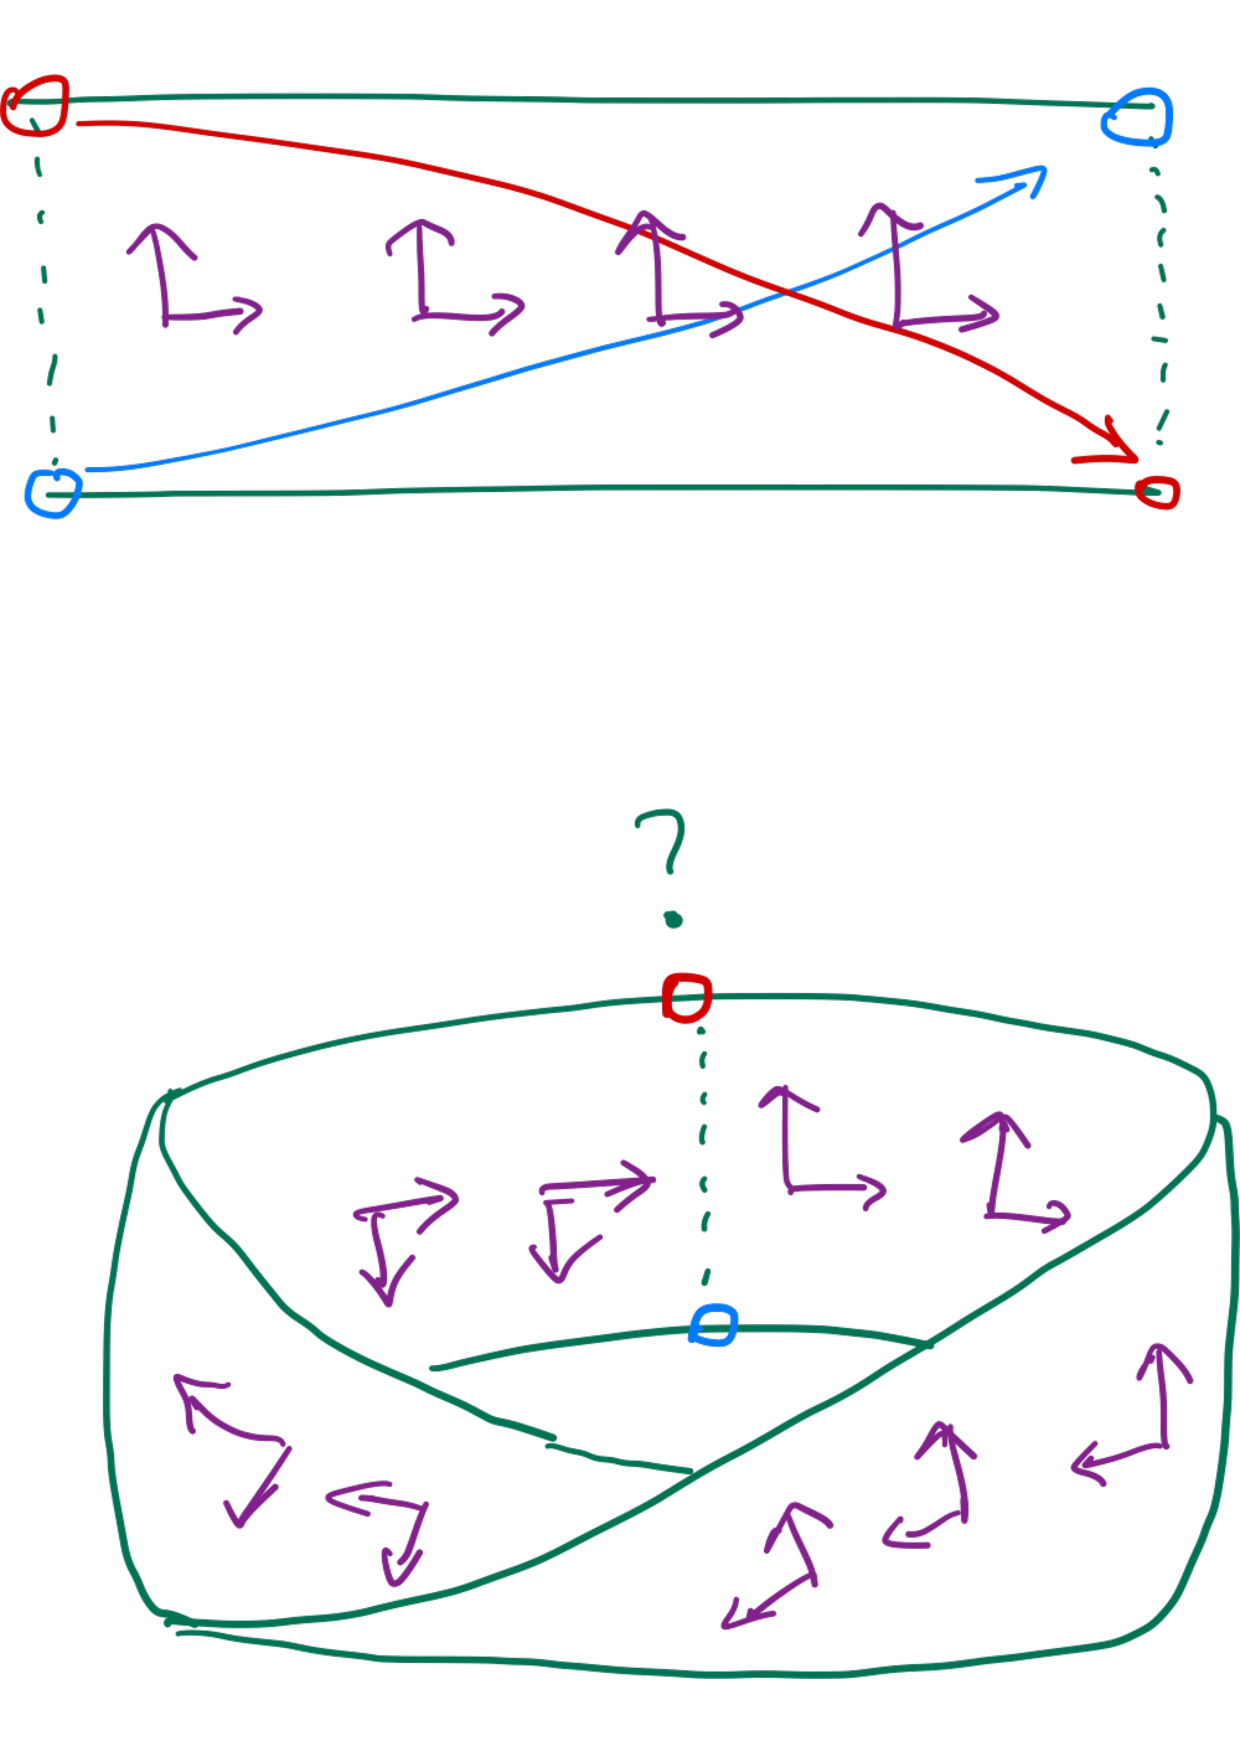
\includegraphics{7_1-mobius_strip.pdf}
\end{marginfigure}

\begin{exercise}
  Consider the open M\"obius strip $M$, a variation of Example~\ref{ex:mobius} defined as the quotient of $\R\times(-1,1)$ via the identification $(x,y) \sim (x+1, -y)$, and denote $\pi: \R\times(-1,1)\to M$ the corresponding projection map.
  The M\"obius strip inherits the differentiable structure from $\R^2$, so we need to show that there is no orientable atlas which is also compatible with the differentiable structure on $M$.
  \begin{enumerate}
    \item Define the map $\sigma:\R\times(-1,1)\to\R\times(-1,1)$ by $\sigma(x,y) = (x+1, -y)$ and show that $\pi\circ\sigma = \pi$.
    \item If $\eta\in\Omega^2(M)$ defines\footnote{Cf. Exercise~\ref{ex:vfshape}.} $f$ by $\pi^* \eta = f \omega$ where $\omega$ is an area\footnote{I.e. a volume $2$-form.} form on $\R\times(-1,1)$.
    Show that $f(x+1, y) = - f(x,y)$.
    \item Conclude that $f$ must vanish at some point of $\R\times(-1,1)$, which implies that $M$ is non-orientable.
  \end{enumerate}
\end{exercise}

\begin{exercise}
  Let $f\in C^\infty(\R^{n+1})$ with $0$ as a regular value.
  Show that $f^{-1}(0)$ is an orientable submanifold of $\R^{n+1}$.
  %In particular, the unit $n$-sphere $\bS^n\subset\R^{n+1}$ is orientable.
\end{exercise}

\begin{remark}
  This definition can be immediately extended to vector bundles.
  Given a real vector bundle $\pi: E \to M$, an orientation of $E$ means that for each fiber $E_p$, there is an orientation of the vector space $E_p$ such that each trivialization map
  \begin{equation}
    \varphi_{U}:\pi^{-1}(U)\to U\times \R^{n},
  \end{equation}
  with $\R^n$ equipped with its standard orientation, is fiberwise orientation-preserving.
  \marginnote[-2em]{Otherwise said, we can cover the manifold by (continuous) local frames whose local trivializations are orientation preserving.}
  With this definition, the orientability of $M$ coincides with the orientability of the bundle $TM\to M$.
\end{remark}

\begin{exercise}\label{ex:TMorient}
  Let $M$ be a smooth manifold without boundary and $\pi: TM \to M$ its tangent bundle.
  Show that if $\{(U_\alpha,\varphi_\alpha)\}$ is any atlas on $M$, then the corresponding\footnote{Remember Theorem~\ref{thm:tgbdlsmoothmfld}.} atlas $\{(TU_\alpha, \widetilde\varphi_\alpha)\}$ on $TM$ is oriented.
  This, in particular, proves that the total space $TM$ of the tangent bundle is always orientable, regardless of the orientability of $M$.
\end{exercise}

A remarkable consequence of Exercise~\ref{ex:TMorient} is that $TM$, as a manifold on its own right, is always orientable, even if $M$ is not. 

\newthought{What about orientation on the boundaries?}

Let's first look at the tangent space. 
If $M$ ia a smooth $n$-manifold with boundary and $p\in \partial M$, we have three types of possible vectors:
\begin{enumerate}
  \item tangent boundary vectors: $X\in T_p(\partial M)\subset T_p M$ tangent to the boundary, forming an $(n-1)$-dimensional subspace of $T_p M$;
  \item inward pointing vectors: $X\in T_pM$ such that $X = \varphi^{-1}_*(Y)$ where $\varphi^{-1}: V\subset \cH^n \to M$ and $Y$ is some vector $Y = (Y_1, \ldots, Y_n)$ with $Y_n > 0$;
  \item outward pointing vectors: $X\in T_pM$ such that $-X$ is inward pointing.
\end{enumerate}
Thus, a vector field along $\partial M$ is a function $X:\partial M\to T_pM$ (not to $T_p\partial M$).

\begin{proposition}
  On a smooth manifold $M$ with boundary, there is a smooth outward pointing vector field along $\partial M$.  
\end{proposition}
\begin{proof}
  Pick an open cover of $\partial M$ with coordinate charts $\{(U_\alpha, (x^1_\alpha,\ldots,x^n_\alpha) \mid \alpha\in I\}$.
  Then $X_\alpha = -\frac{\partial}{\partial x^n_\alpha}$ on $U_\alpha\cap \partial M$ is smooth and outward pointing.
  Choose a partition of unity $\{\rho_\alpha \mid \alpha\in I\}$ on $\partial M$ subordinate to the open cover $\{U_\alpha\cap \partial M \mid \alpha\in I\}$.
  Then $X:= \sum_{\alpha\in I}\rho_\alpha X_\alpha$ is a smooth ouwtard pointing vector field along $\partial M$.
\end{proof}

We can use this to introduce a notion of induced orientation on $\partial M$.

\begin{proposition}
  Let $M$ be an oriented $n$-manifold with boundary.
  If $\omega$ is a volume form on $M$ and $X$ a smooth outward-pointing vector field on $\partial M$, then $\iota_X\omega$ is a smooth nowhere-vanishing $(n-1)$-form on $\partial M$ and, thus, $\partial M$ is orientable.
\end{proposition}
\begin{proof}
  Since both $\omega$ and $X$ are smooth, the contraction $\iota_X\omega$ is also smooth.
  We need to check that it cannot vanish.

  Assume that $\iota_X\omega$ does vanish at some point $p\in\partial M$, that is, $(\iota_X)(v_1, \ldots, v_{n-1}) = 0$ for all $v_1, \ldots, v_{n-1}\in T_p(\partial M)$.
  Let $\{e_1,\ldots,e_{n-1}\}$ be a basis for $T_p(\partial M)$.
  Then $\{X_p,e_1,\ldots,e_{n-1}\}$ is a basis for $T_p M$ such that
  \begin{equation}
    \omega_p(X_p, e_1, \ldots, e_{n-1}) = (\iota_X\omega)_p(e_1, \ldots, e_{n-1}) = 0.
  \end{equation}
  Then, by Exercise~\ref{ex:zeroform}, $\omega_p\equiv0$ reaching a contradiction.
  
  Therefore, $\iota_X\omega$ is non-vanishing on $\partial M$ which means that $\partial M$ is orientable.
\end{proof}

\begin{exercise}\label{ex:vfshape}
  Let $M$ be an oriented manifold with boundary, $\omega$ an orientation for $M$ and $X$ a smooth outward pointing vector field along $\partial M$.
  Prove the following statements.
  \begin{enumerate}
    \item It $\sigma$ is another orientation form on $M$, then $\sigma = f\omega$ for some everywhere positive $f\in C^\infty(M)$. Prove that  $\iota_X\sigma = f\iota_X \omega$ on $\partial M$.
    \item Show that if $Y$ is another smooth outward pointing vector field along $\partial M$, then there is an everywhere positive $f\in C^\infty(M)$ such that $\iota_Y\sigma = f \iota_X \omega$ on $\partial M$.
  \end{enumerate}
\end{exercise}

Note that if $\{(U_i, \varphi_i)\}$ is a positively oriented atlas on $M$, then $\{(U_i|_{\partial M}, \varphi_i|_{\partial M})\}$ can be negatively oriented. 
Let $\omega = dx^1\wedge\cdots\wedge dx^n$ be a positive volume form on $M$ on one of the charts, then $-\frac{\partial}{\partial x^n}$ is an outward pointing on $\partial \cH^n$ and we have\footnote{Recall Lemma~\ref{lemma:intprod}.}
\begin{align}
  \iota_{-{\partial}/\!{\partial x^n}} (dx^1\wedge\cdots\wedge dx^n)
  &= -\iota_{{\partial}/\!{\partial x^n}} (dx^1\wedge\cdots\wedge dx^n) \\
  &= -(-1)^{n-1} dx^1\wedge\cdots\wedge dx^{n-1}\wedge \iota_{{\partial}/\!{\partial x^n}} (dx^n) \\
  &= (-1)^n dx^1\wedge\cdots\wedge dx^{n-1}.
\end{align}
Thus, for example, the boundary orientation on $\partial \cH^1 = \{0\}$ is $-1$, the one on $\partial \cH^2$ is the standard orientation on $\R$ given by $dx^1$ and the one on $\partial \cH^3$ is $-dx^1\wedge dx^2$, which is the clockwise orientation in the $(x^1, x^2)$-plane, etc.

\begin{example}\label{ex:int:bdryo}
  The closed interval $[a,b]\subset\R$ with standard euclidean coordinate $x$ has a standard orientation given by the vector field $\frac{\partial}{\partial x}$. 
  Therefore\footnote{Recall the charts in Example~\ref{ex:mfldbdryinterval}.}, the boundary orientation at $b$ is $\iota_{\frac{\partial}{\partial x}}(dx) = +1$ and the one at $a$ is $\iota_{-\frac{\partial}{\partial x}}(dx) = -1$.
\end{example}

\begin{exercise}
  Orientability is common but there are many examples of nonorientable manifolds.
  \begin{enumerate}
    \item Prove that $\bS^n$ is orientable.\\
      \textit{\small Hint: above there is a small exercise that can help a lot here.}
    \item Prove that any Lie group is orientable.
    \item Prove that $\RP^n$ is orientable if and only if $n$ is odd. \\
      \textit{\small Hint: the antipodal map $x\mapsto -x$ on $\bS^n$ can help.}
  \end{enumerate}
\end{exercise}

\section{Integrals on manifolds}

To avoid unnecessary complications, we will only integrate $n$-forms with compact support.
Armed with our experience with line integrals, fond memories of multivariable analysis and our recent discoveries, we are finally ready to talk about integrals.
Let's keep things simple and go one step at a time.

\begin{definition}\label{def:intnform:chart}
  Let $M$ be a smooth $n$-manifold and $(U,\varphi)$ be a chart from an oriented atlas of $M$ with coordinates $(x^i)$.
  If $\omega\in\Omega^n(M)$ be a $n$-form, $n > 0$, with compact support in $U$, we define the integral of $\omega$ as\footnote{Recall that for a diffeomorphism $\phi$, $\phi_* = (\phi^{-1})^*$.}
  \begin{equation}
    \int_M \omega = \int_U \omega := \int_{\varphi(U)} \varphi_*\omega := \int_{\R^n} \omega(x) d x^1\cdots dx^n,
  \end{equation}
  where the last is the usual Riemannian integral on $\R^n$ and, on the chart,
  \begin{equation}
    \varphi_*\omega = \omega(x)\; dx^{1}\wedge \cdots\wedge dx^{n}\in\Omega^n(\R^n).
  \end{equation}
  For convenience we may write $d^n x := dx^1 \cdots dx^n$.
  \marginnote[-5em]{Everything remains valid if $\R^n$ is replaced by $\cH^n$.}

  If $M$ is an oriented $0$-dimensional manifold and $f\in\Omega^0(M) = C^\infty(M)$, than we define the integral to be the sum
  \begin{equation}
    \int_M f := \sum_{p\in M} \pm f(p),
  \end{equation}
  where we take the positive sign at points where the orientation is positive and the negative sign at points where it is negative.
  The compactness assumption here implies that there are only finitely many nonzero terms in the sum.
\end{definition}

To make sure that this definition makes sense, let's show that the integral is well-defined, that is, up to orientation it does not depend on the chosen chart.

\begin{lemma}\label{lemma:intindep:chart}
  Suppose $\omega\in\Omega^n(M)$ with compact support $\supp \omega \subset U\cap V$, where $(U, \varphi)$ and $(V, \psi)$ are two positively oriented charts on the oriented manifold $M$.
  Then, the value of the integral $\int_M\omega$ is independent on the chosen chart.
\end{lemma}
\begin{proof}
  Let $\varphi$ and $\psi$ be two charts on $W = U\cap V$ with the same orientation and local coordinates $x$ and $y$, let $\sigma = \psi\circ\varphi^{-1}$ be the corresponding transition map.
  Denote, locally, $\varphi_*\omega = \omega(x) dx^1\wedge\cdots\wedge dx^n$ and $\psi_*\omega = \widetilde\omega(y) dy^1\wedge\cdots\wedge dy^n$.
  Then,
  \marginnote{Since in multivariable analysis you saw already the invariance of the Euclidean integral by orientation-preserving changes of coordinates, one could also use that directly:
  \begin{align}
    \int_{\varphi(U)} \varphi_*\omega & = \int_{\varphi(W)} \varphi_*\omega \\
    &= \int_{\sigma(\varphi(W))} \sigma_* (\varphi_*\omega) \\
    &= \int_{\psi(W)} \psi_* \omega.
  \end{align}
  }
  \begin{align}
    \int_{\varphi(W)} \varphi_*\omega &= \int \omega(x)\, d^n x \\
    &\overset{\eqref{form:cov}}{=} \int_{\varphi(W)} (\widetilde\omega \circ \sigma)(x) \det(D\sigma|_x) d^n x \\
    &\overset{(\clubsuit)}{=} \int_{\psi(W)} \widetilde\omega(y) d^n y\\
    &= \int_{\psi(W)} \psi_*\omega,
  \end{align}
  where in $(\clubsuit)$ we used the classical euclidean change of variables.
\end{proof}

To be able to integrate charts which are not supported in the domain of a single chart, we now need the help of a partition of unity.

\begin{definition}
  Let $M$ be a smooth oriented manifold and $\cA = \{(U_i,\varphi_i)\}$ a positively oriented atlas.
  If $\omega \in \Omega^n(M)$ has compact support, then the \emph{integral of $\omega$} is defined as
  \begin{equation}\label{eq:intnform}
    \int_M \omega := \sum_{j=1}^N \int_{U_j}\rho_j\omega,
  \end{equation}
  where $\{\rho_j\mid j=1,\ldots, N\}$ is a partition of unity subordinate to a finite cover\footnote{Such that $\sum_{j=1}^N \rho_j(p) = 1$ for $p\in\supp\omega$.} of $\supp \omega$ by charts domains $\{U_j\}$.
  \marginnote[-7em]{The terms on the right hand side of \eqref{eq:intnform} are all integrals as in Definition~\ref{def:intnform:chart}.}
\end{definition}

The definition above makes sense only if the value of the integral is independent of the chosen partition, but with the help of the previous lemma this is easily checked.

\begin{lemma}\label{lemma:intinman}
  The value of $\int_M\omega$ is independent from the choice of the atlas and the choice of partition of unity.
\end{lemma}
\begin{proof}
  The independence from the choice of the charts was demonstrated in Lemma~\ref{lemma:intindep:chart}.
  Let $\{\widetilde\rho_j\}$ be another partition of unity subordinate to a (possibly different) finite cover by charts $\{(V_j, \psi_j)\}$ with $\sum \widetilde\rho_j(p) = 1$ for $p\in\supp\omega$.
  Then we have,
  \begin{align}
    \sum_j \int_{\varphi_j(U_j)} (\varphi_j)_*\left(\rho_j \omega\right)
    &= \sum_j \int_{\varphi_j(U_j)} (\varphi_j)_*\left(\rho_j \sum_k \widetilde\rho_k\omega\right) \\
    &= \sum_{j,k} \int_{\varphi_j(U_j\cap V_k)} (\varphi_j)_* \left(\rho_j \widetilde\rho_k\omega\right) \\
    &\overset{(\spadesuit)}{=} \sum_{j,k} \int_{\psi_k(U_j\cap V_k)} (\psi_k)_* \left(\rho_j \widetilde\rho_k\omega\right) \\
    &= \sum_k \int_{\psi_k(V_k)} (\psi_k)_*\left(\widetilde\rho_k \sum_j\rho_j \omega\right) \\
    &= \sum_k \int_{\psi_k(V_k)} (\psi_k)_*\left( \widetilde\rho_k \omega\right),
  \end{align}
  where in $(\spadesuit)$ we used Lemma~\ref{lemma:intindep:chart}.
\end{proof}

Which immediately implies the following nice result.
\begin{theorem}[Global change of variables]\label{thm:gcv}
  Suppose $M$ and $N$ are oriented $n$-manifolds and $F:M\to N$ is an orientation preserving diffeomorphism.
  If $\omega\in\Omega^n(N)$ has compact support, then $F^*\omega$ has compact support and the following holds
  \begin{equation}
    \int_N \omega = \int_M F^* \omega.
  \end{equation}
\end{theorem}
\begin{proof}
  First of all, observe that $\supp(F^*\omega) = F^{-1}(\supp(\omega))$ which is compact since manifolds are Hausdorff spaces and $F$ is continuous.

  Let now $\{(U_i,\varphi_i)\}$ be an atlas of a positively oriented chart on $M$ and $\{\rho_i\}$ a subordinate partition of unity.
  Then, $\{(F(U_i),\varphi_i\circ F^{-1})\}$ is an atlas of positively oriented charts for $N$ and $\{\rho_i \circ F^{-1}\}$ is a partition of unity subordinate to the covering $\{F(U_i)\}$.
  By Lemma~\ref{lemma:intinman} we have,
  \begin{align}
    \int_M F^*\omega &= \sum_i \int_M \rho_i F^*\omega \\
    &= \sum_i \int_{\R^n}(\varphi_i)_*(\rho_i F^*\omega)\\
    &= \sum_i \int_{\R^n}(\varphi_i)_*(F^{-1})_*(\rho_i \circ F^{-1}) \omega \\
    &= \sum_i \int_{\R^n}(\varphi_i \circ F^{-1})_*(\rho_i \circ F^{-1}) \omega \\
    &= \int_N\omega,
  \end{align}
  which shows the commutativity of the following diagram
  \begin{equation}
    \begin{tikzcd}
      \Omega^n(M)
        \arrow[rr, "F^*", above, shift right = 0.5]
        \arrow[dr, "\int_M", below left]
        & & \Omega^n(N)
          \arrow[ll, "F_*", below, shift right = 0.5]
          \arrow[dl, "\int_N"] \\
      & \R &
    \end{tikzcd}
  \end{equation}
  and concludes the proof.
\end{proof}

This justifies the following definition.

\begin{definition}[Integral on submanifolds]\label{def:insm}
  Let $M$ an oriented smooth $m$-manifold, $N$ an oriented smooth $n$-manifold and $J:N\to M$ a smooth map\footnote{If $N\subset M$ is a submanifold, then $J:N\hookrightarrow M$ is just the inclusion map.}.
  If $\omega\in\Omega^n(M)$ restricted to $J(N)$ has compact support, we define
  \begin{equation}
    \int_N \omega := \int_N J^*\omega.
  \end{equation}
  In particular, if $M$ is compact, oriented, smooth $m$-manifold, $\omega\in\Omega^{m-1}(M)$ and $i:\partial M\hookrightarrow M$ is the inclusion of the boundary in $M$, we can interpret unambiguously
  \begin{equation}
    \int_{\partial M} \omega := \int_{\partial M} i^* \omega,
  \end{equation}
  where $\partial M$ is understood to have the induced orientation.
\end{definition}

\begin{example}\label{ex:intint}
  Let $M=[a,b]\subset \R$ equipped with the canonical global atlas $\{(M, \id_\R|_M)\}$ and $f\in C^\infty_0(M)$, i.e., smooth with compact support\footnote{Which does not mean $f(a) = f(b)=0$ since $[a,b]$ is itself compact.}.
  Then, $df\in\Omega^1(M)$ and $\supp df \subset \supp f$ is compact as well and we have
  \begin{equation}
    \int_M df = \int_a^b \frac{\partial f}{\partial x} dx = f(b)- f(a) = \int_{\partial M} f.
  \end{equation}
\end{example}

\begin{exercise}[Fubini's theorem]\label{exe:fubini}
  Let $M^m$ and $N^n$ be oriented manifolds. Endow $M\times N$ with the product orientation, that is\footnote{An equivalent way is to say that if $v_1,\ldots,v_m\in T_pM$ and $w_1, \ldots, w_n\in T_q N$ are positively oriented bases in the respective spaces, then \begin{equation}
    (v_1,0),\ldots,(v_n,0),(0,w_1), \ldots, (0,w_n)\in T_{(p,q)}(M\times N)
  \end{equation}is defined to be a positively oriented basis in the product.}, if $\pi_M : M\times N \to M$ and $\pi_N: M\times N \to N$ are the canonical projections on the elements of the product, and $\omega$ and $\eta$ respectively define orientations on $M$ and $N$, then the orientation on $M\times N$ is defined to be the orientation defined by $\pi_M^* \omega \wedge \pi_N^* \eta$.

  If $\alpha\in\Omega^m(M)$ and $\beta\in\Omega^n(N)$ have compact support, show that
  \begin{equation}
    \alpha\times\beta := (\pi_M^*\alpha)\wedge(\pi_N^*\beta)
  \end{equation}
  has compact support and is a $(m+n)$-form on $M\times N$.
  Then, prove Fubini's theorem:
  \begin{equation}
    \int_{M\times N}\alpha\times\beta = \left(\int_M\alpha\right)\left(\int_N\beta\right).
  \end{equation}
\end{exercise}

\begin{exercise}
  Let $\{e_1,\ldots,e_{n+1}\}$ be the standard basis of $\R^{n+1}$ and $\Omega_{n+1} := e_1\wedge\cdots\wedge e_{n+1}$ the induced volume form.
  On $\bS^n$ define $\omega_n\in\Omega^n(\bS^n)$ by
  \begin{equation}
    \omega_n(s)(v_1, \ldots, v_n) = \Omega_{n+1}(s, v_1, \ldots, v_n)
  \end{equation}
  for $s\in\bS^n$ and $v_1,\ldots,v_n\in T_s\bS^n$.

  In this exercise we are going to define a canonical volume $\omega_n$ on $\bS^n$ and prove that 
  \begin{equation}
    \int_{\bS^n} \omega_n = \frac{2^{m+1}\pi^m}{(2m-1)!}, \quad\mbox{if } n=2m,\; m\geq 1,
  \end{equation}
  and
  \begin{equation}
    \int_{\bS^n} \omega_n = \frac{2\pi^{m+1}}{m!}, \quad\mbox{if } n=2m+1,\; m\geq 0.
  \end{equation}

  \begin{enumerate}
    \item Show that $\omega_n$ is a volume form on $\bS^n$. In fact it is the so-called standard volume form on $\bS^n$.
    \item Let $f:\R_+\times\R^{n+1}\setminus\{0\}\to \R^{n+1}\setminus\{0\}$ be given by $f(t,s) = ts$, where $\R_+$ is defined to be the set $\{t\in\R \mid t >0\}$.
    Show that if $\R_+$ is oriented by $dt$, $\bS^n$ is oriented by $\omega_n$ and $\R^{n+1}$ is oriented by $\Omega_{n+1}$, then the Jacobian determinant $\det(Df(t,s))= t^n$.
    Conclude that $f$ is orientation preserving.
    \item Let $M$ be the annulus $M = \{x\in\R^{n+1} \mid 0<a<\|x\|<b<\infty\}$. Consider the restriction $f|_{(a,b)\times \bS^n}$ and show that for $x\in\R^{n+1}$,
    \begin{equation}
      f^*\left(e^{-\|x\|^2}\Omega_{n+1}\right) = t^n e^{-t^2}(dt \times \omega_n),
    \end{equation}
    where $dt\times\omega_n$ is a product volume form as in Exercise~\ref{exe:fubini}.
    \item Show that
    \begin{equation}
      \int_{\R^{n+1}}e^{-\|x\|^2}\Omega_{n+1} = \int_a^b t^ne^{-t^2} dt \int_{\bS^n}\omega_n.
    \end{equation}
    \item Consider the limits $a\to0^+$ and $b\to+\infty$ and show that
    \begin{equation}
      \int_0^\infty t^n e^{-t^2} dt \int_{\bS^n}\omega_n = \left(\int_{-\infty}^{+\infty} e^{-u^2} du\right)^{n+1}.
    \end{equation}
    \item Assume to know that $\int_{-\infty}^{\infty} e^{-u^2}du = \sqrt{\pi}$. Show that
    \begin{equation}
      \int_0^\infty t^{2m} e^{-t^2}dt = \frac{(2m-1)!!\sqrt{\pi}}{2^{m+1}}
      \quad\mbox{and}\quad
      \int_0^\infty t^{2m+1} e^{-t^2}dt = \frac{m!}{2},
    \end{equation}
    and use them to deduce the required formulas for $\int_{\bS^n}\omega_n$.
  \end{enumerate}
\end{exercise}

\begin{corollary}[Of Theorem~\ref{thm:gcv}]
  Let $F:M\to M$ be a diffeomorphism and $\omega\in\Omega^n(M)$ an invariant volume form, that is, $F^*\omega =\omega$.
  Then, for all compactly supported smooth functions $f\in C^\infty_0(M)$, the following holds
  \begin{equation}
    \int_M f\omega = \int_M (f\circ F)\omega.
  \end{equation}
\end{corollary}
\begin{proof}
  Follows form the previous exercise by observing
  \begin{equation}
    F^*(f\omega) = (f\circ F) F^*\omega = (f\circ F)\omega.
  \end{equation}
\end{proof}

This corollary has deep consequences in classical mechanics, which I am going to teach in the master and you are welcome to attend!

\begin{remark}
  The integral defined in this section can be extended rather immediately to measurable functions.
  Let $\omega\in\Omega^n(M)$ be a positive volume form and let $f:M\to[0,\infty)$ be measurable.
  Then one can define
  \begin{align}
    \int_M f \omega
    &= \sum_i \int_{\varphi_i(U_i)} (\varphi_i)_*(\rho_i f\omega) \\
    &= \sum_i \int_{\varphi_i(U_i)} (\rho_i f \circ\varphi_i^{-1}) (\varphi_i)_*\omega \\
    &= \sum_i \int_{\varphi_i(U_i)} (\rho_i f \circ\varphi_i^{-1})(x) \omega(x) d^n x,
  \end{align}
  where the last integral is a Lebesgue integral on $\R^n$.
  One then calls $f:M\to \R$ integrable, saying $f\in L^1(M,\omega)$, if $\int_M|f|\omega < \infty$ and defines its integral as $\int_M f\omega := \int_M f^+\omega - \int_M f^-\omega$, where $f^\pm$ denote the positive and negative components of $f$ as in the euclidean case.
\end{remark}

\section{Stokes' Theorem}

Stokes' theorem states that if $\omega$ is an $(n-1)$-form on an orientable $n$-manifold $M$, then the integral of $d\omega$ over $M$ equals the integral of $\omega$ over $\partial M$, generalising our observations for the line integral.
This is a beautiful and very important results, with deep consequences. The most immediate ones are the classical theorems of Gauss, Green and Stokes, which are just a special cases of this result.

We are going to state the theorem, discuss some of its consequences and then give its proof.

\begin{theorem}[Stokes' theorem]\label{thm:Stokes}
  Let $M$ be an oriented $n$-manifold with boundary and let $\omega\in\Omega^{n-1}(M)$ be compactly supported.
  Then,
  \begin{equation}\label{eq:Stokes}
    \int_M d\omega = \int_{\partial M} \omega.
  \end{equation}
  \marginnote[-4.5em]{Here, $\partial M$ inherits the orientation from $M$ as in Definition~\ref{def:insm}, $\omega$ on the right-hand side is interpreted as $i^*\omega$ where $i:\partial M \hookrightarrow M$ is the inclusion of the boundary and if $\partial M =\emptyset$ then the right-hand side is interpreted as $0$.}
\end{theorem}

\marginnote[1em]{On a similar note, the fact that $dd\omega =0$ for every $\omega\in\Lambda^n(M)$ corresponds to the fact that a boundary has no boundary, that is $\partial\partial M = \emptyset$ for any $M$: indeed, for any $\omega\in\Lambda^n(M)$ one has \begin{equation}
  0=\int_M dd\omega = \int_{\partial M}d\omega = \int_{\partial\partial M} \omega.
\end{equation}}
\begin{corollary}
  Let $M$ be an oriented $n$-manifold without boundary and let $\omega\in\Omega^{n-1}(M)$ be compactly supported.
  Then,
  \begin{equation}
    \int_M d\omega = 0.
  \end{equation}
  That is, the integral of a compactly supported exact form over a manifold without boundary vanishes.
\end{corollary}

\begin{corollary}
  Let $M$ be a compact oriented $n$-manifold with boundary and let $\omega\in\Omega^{n-1}(M)$ be closed.
  Then,
  \begin{equation}
    \int_{\partial M} \omega = 0.
  \end{equation}
  That is, the integral of a closed form on the boundary of a compact manifold vanishes.
\end{corollary}

\begin{corollary}
  Let $M$ a smooth $m$-manifold, $N$ an oriented smooth $n$-manifold and $J:N\to M$ a smooth map\footnote{If $N\subset M$ is a submanifold, then $J:N\hookrightarrow M$ is just the inclusion map.}.
  If $\omega\in\Omega^{n-1}(M)$ restricted to $J(N)$ has compact support, then
  \begin{equation}
    \int_{N} d J^*\omega = \int_{\partial N} J^*\omega,
  \end{equation}
  where $\partial N$ inherits the orientation of $N$.
\end{corollary}

\begin{corollary}[Green's theorem]
  Suppose $D$ is a compact regular domain in $\R^2$ and $P,Q\in C^\infty(D)$, then
  \begin{equation}
    \int_D \left(\frac{\partial Q}{\partial x} - \frac{\partial P}{\partial y}\right)dxdy = \int_{\partial D}(Pdx + Qdy).
  \end{equation}
\end{corollary}

\begin{remark}
  The requirement of compactness in Stokes' theorem may seem there just to avoid technicalities involving the convergence of the integral, however, it also avoid subtleties due to the boundary as shown in the following example.
  Let $M=(a,b)$, thus $\partial M = \emptyset$, and $f(x)=x$.
  Then,
  \begin{equation}
    b-a = \int_a^b df \neq \int_{\partial M} f = 0.
  \end{equation}
  But this does not contradict Stokes' theorem since $f$ is not compactly supported.

  If you close the interval, then $f$ becomes with compact support and we are back in the case of Example~\ref{ex:intint} where we had already seen Stokes' theorem.
\end{remark}

\begin{proof}
  \newthought{Part I: euclidean boundary case}.
  Let's start with a special case: suppose $M = \cH^n$ itself.
  Since $\omega$ has compact support, there is $R > 0$ such that $\supp \omega \subset A = [-R,R]^{n-1}\times[0,R]$ is enclosed within the rectangle $A$.
  We can write $\omega$ in standard coordinates to get
  \begin{equation}
    \omega = \sum_{j=1}^n \omega^j dx^1 \wedge \cdots\wedge \widehat{dx}^j \wedge \cdots\wedge dx^n
  \end{equation}
  where the hat means that the corresponding element $dx^j$ is omitted.
  Therefore\footnote{Exercise: explicitly write down the steps of the computation.},
  \begin{equation}
    d\omega = \sum_{j=1}^n (-1)^{j-1} \frac{\partial \omega^j}{\partial x^j}dx^1\wedge\cdots\wedge dx^n,
  \end{equation}
  and we end up with the integral
  \begin{align}
    \int_{\cH^n} d\omega
    &= \sum_{j=1}^n (-1)^{j-1} \int_A\frac{\partial \omega^j}{\partial x^j}dx^1\wedge\cdots\wedge dx^n \\
    &= \sum_{j=1}^n (-1)^{j-1} \int_0^R\int_{-R}^R\cdots\int_{-R}^{R}\frac{\partial \omega^j}{\partial x^j}(x) d^n x. %d x^1\cdots dx^n.
  \end{align}
  The last are genuine euclidean integrals and we can change the order of integration in each term to always integrate the $x^j$ term first.
  The usual euclidean fundamental theorem of calculus then, for the terms with $j\neq n$, implies
  \begin{align}
    \int_{\cH^n} d\omega
    &= \sum_{j=1}^n (-1)^{j-1} \int_0^R\int_{-R}^R\cdots\int_{-R}^{R}\frac{\partial \omega^j}{\partial x^j}(x) d^n x \\ %dx^1\cdots dx^n \\
    &=\sum_{j=1}^n (-1)^{j-1} \int_0^R\int_{-R}^R\cdots\int_{-R}^{R}\frac{\partial \omega^j}{\partial x^j}(x) dx^j dx^1\cdots\widehat{dx^j}\cdots dx^n \\
    &=\sum_{j=1}^n (-1)^{j-1} \int_0^R\int_{-R}^R\cdots\int_{-R}^{R}\omega^j(x) \Big|_{x^j=-R}^{x^j=R} dx^1\cdots\widehat{dx^j}\cdots dx^n \\
    &= 0
  \end{align}
  since $R$ is larger than the support of $\omega$ at each coordinate.
  The only term that may not be zero is the $j=n$ one.
  In that case, for the same reasons,
  \begin{align}
    \int_{\cH^n} d\omega
    &=(-1)^{n-1} \int_{-R}^R\int_{-R}^R\cdots\int_{-R}^R\int_{0}^{R}\frac{\partial \omega^n}{\partial x^j}(x) dx^n d^{n-1} x \\ %dx^1\cdots dx^{n-1} \\
    &=(-1)^{n-1} \int_{-R}^R\int_{-R}^R\cdots\int_{-R}^R \omega^n(x)\Big|_{x^n=0}^{x^n=R} dx^n d^{n-1} x \\ %dx^1\cdots dx^{n-1} \\
    &=(-1)^{n-1} \int_{-R}^R\int_{-R}^R\cdots\int_{-R}^R \omega^n(x^1, \ldots, x^{n-1}, 0) d^{n-1} x %dx^1\cdots dx^{n-1}.
    .\label{eq:lhsHn}
  \end{align}
  We now need to compare this with the right-hand side of~\eqref{eq:Stokes}.
  To this end, compute he following
  \begin{equation}
    \int_{\partial \cH^n}\omega = \sum_{j=1}^n \int_{A\cap\cH^n} \omega_j(x^1, \ldots, x^{n-1}, 0) dx^1 \wedge \cdots\wedge \widehat{dx}^j \wedge \cdots\wedge dx^n.
  \end{equation}
  Since $x^n$ vanishes on $\partial\cH^n$, the pullback of $dx^n$ to the boundary is zero, and thus the only surviving term in the sum is the last one, that is,
  \begin{equation}\label{eq:rhsHn}
    \int_{\partial \cH^n}\omega = \int_{A\cap\cH^n} \omega_n(x^1, \ldots, x^{n-1}, 0) dx^1 \wedge\cdots\wedge dx^{n-1}.
  \end{equation}
  Since coordinates $(x^1, \ldots, x^{n-1})$ are positively oriented for $\cH^n$ when $n$ is even and negatively oriented when $n$ is odd, we obtain the equality of \eqref{eq:lhsHn} and \eqref{eq:rhsHn}.

  \newthought{Part II: euclidean case}.
  If $M=\R^n$ the considerations above apply without the need to make an exception for the case $j=n$, so all the terms vanish on the left-hand side of~\eqref{eq:Stokes} while the right-hand side is trivially zero due to the empty boundary.

  \newthought{Part III: ``arbitrary'' $M$ but $\supp\omega$ is contained in a single chart}.
  Let $(U,\varphi)$ denote a chart such that $\supp \omega \subset U$.
  Without loss of generality assume that $\varphi$ is a positively oriented boundary chart, then
  \begin{align}
    \int_M d\omega
    &= \int_{\cH^n}(\phi^{-1})^* dw \\
    &= \int_{\cH^n} d\left((\phi^{-1})^* \omega\right) \\
    &\overset{(\spadesuit)}{=} \int_{\partial \cH^n}(\phi^{-1})^* w \\
    &= \int_{\partial M} w , 
  \end{align}
  where in the $(\spadesuit)$ step we applied the computations above and where $\partial \cH^n$ has the orientation induced by $\cH^n$.
  For a negatively oriented smooth boundary chart, the computation applies with an extra negative sign on each side of the equation.
  For an interior chart, we get the same computations with $\R^n$ in place of $\cH^n$.

  \newthought{Part IV: ``arbitrary'' $M$ and $\omega$}.
  Let finally $\omega\in\Omega^{n-1}(M)$ with compact support.
  Without loss of generality, let $\{(U_i, \varphi_i)\mid i\in I\}$ be a finite cover of $\supp \omega$ by positively oriented charts and $\{\rho_i\}$ a subordinate partition of unity with $\sum \rho_i(p) = 1$ for all $p\in\supp \omega$.
  Then, by applying the previous arguments for each $i$ we get
  \begin{align}
    \int_{\partial M} \omega
    &= \sum_i \int_{\partial M} \rho_i\omega
     = \sum_i \int_M d(\rho_i \omega) \\
    &= \sum_i \int_M (d\rho_i \wedge\omega + \rho_i\, d\omega) \\
    &= \int_M d\left(\sum_i \rho_i\right)\wedge\omega + \int_M \left(\sum_i \rho_i\right) d\omega \\ 
    &= 0 + \int_M d\omega,
  \end{align}
  concluding the proof.
\end{proof}

\begin{exercise}
  Let $D^n := \{x=(x^1, \ldots, x^n)\in\R^n \mid \|x\| \leq 1\}$ denote the unit disk in $\R^n$ centred at $0$. Recall that $\partial D^n = \bS^{n-1}$.
  \begin{enumerate}
    \item Compute $\int_{\bS^1} \eta$ where $\eta$ is the following 1-form on $\R^2$: $\eta = -x^2 dx^1 + x^1 dx^2$.
    \item Compute $\int_{\bS^2} \omega$ where $\omega$ is the following 2-form on $\R^3$: $\omega = -x^1 dx^1\wedge dx^3 - x^2 dx^1\wedge dx^3 + x^3 dx^1\wedge dx^2$.
    \item Show that $\eta$ and $\omega$ above are closed but not exact (as differential forms on $\bS^1$ and $\bS^2$ respectively).
  \end{enumerate}
  \textit{\small Hint: if you look carefully, you may notice that you don't really need to write anything down in coordinates.}
\end{exercise}

\begin{example}
  Consider the annulus $M=\{(x,y)\in\R^2 \mid 1/2\leq x^2+y^2 \leq 1\}$ and the $1$-form $\omega = \frac{-y dx + x dy}{x^2 + y^2} = d\theta$ where $(x,y) = (\rho\cos\theta, \rho\sin\theta)$.
  
  Then $d\omega = 0$ and therefore $\int_M d\omega = 0$.
  Furthermore,
  \begin{marginfigure}
    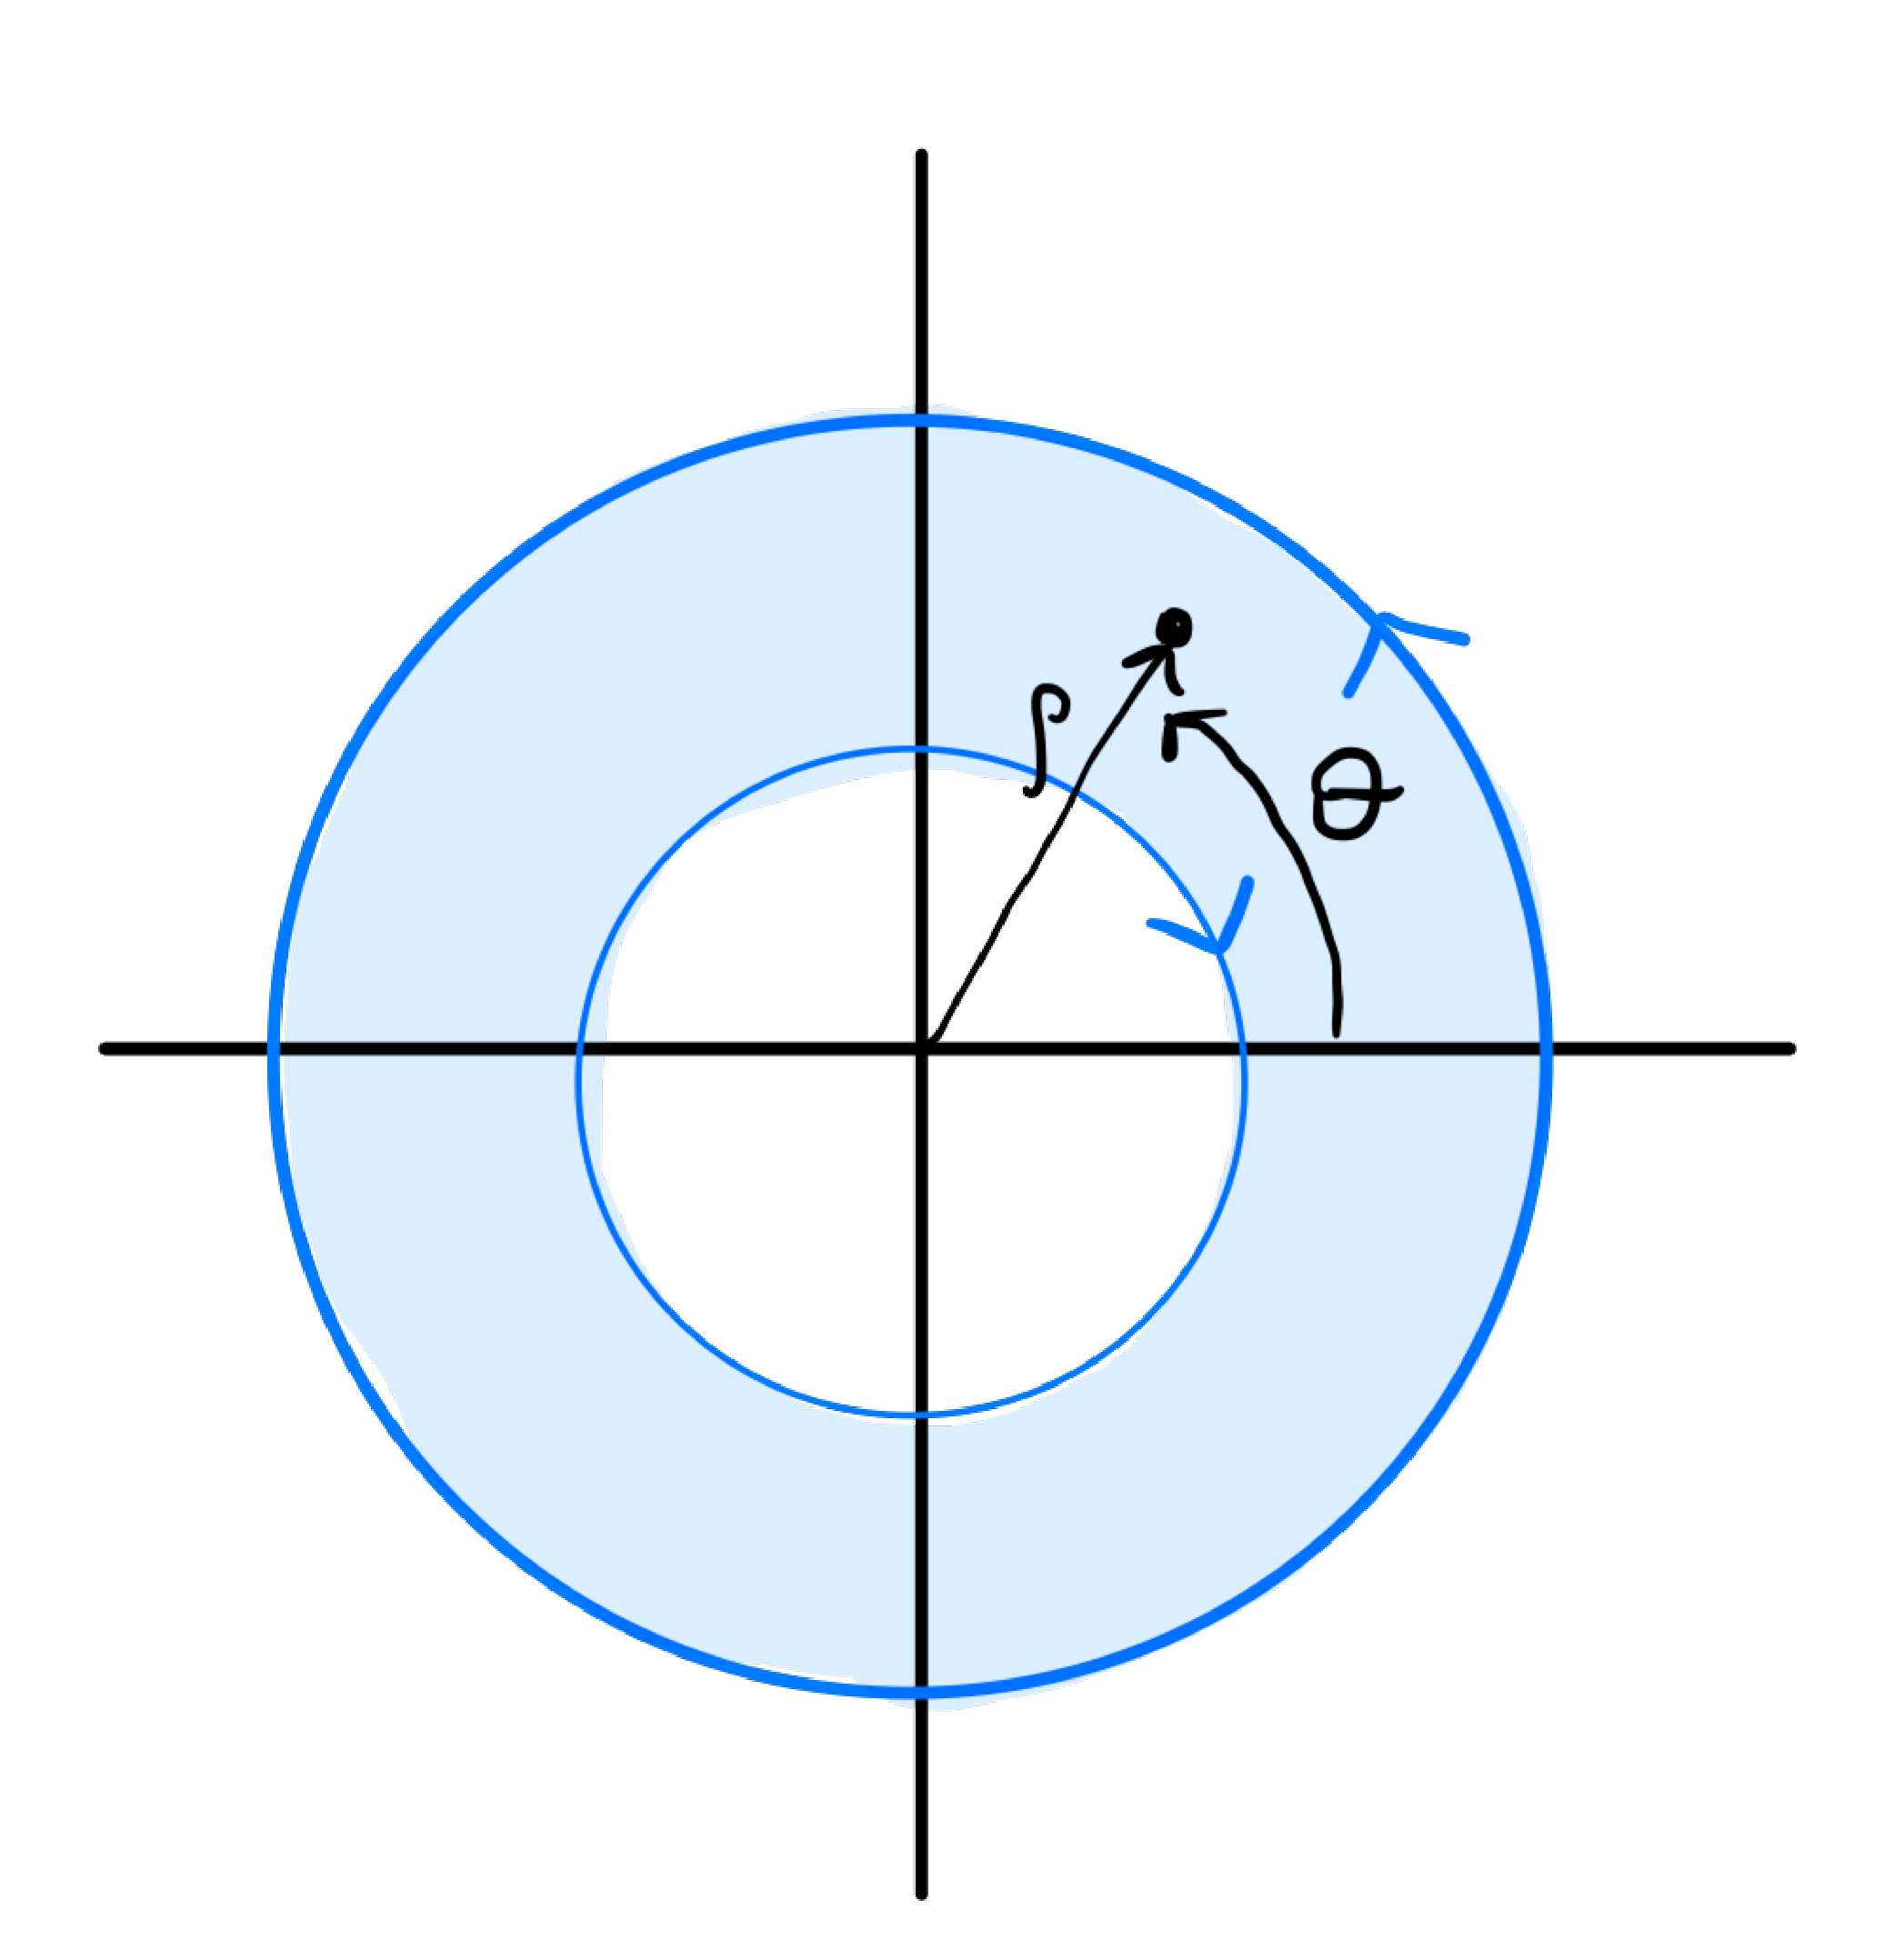
\includegraphics{8_3_8-annulus.pdf}
  \end{marginfigure}
  \begin{align}
    \int_{\partial M}\omega
    &= \int_{x^2 + y^2 =1} \omega + \int_{x^2+y^2 =1/2}\omega \\ 
    &= \int_{0}^{2\pi} d\theta - \int_0^{2\pi}d \theta \\
    &= 2\pi - 2\pi = 0.
  \end{align}

  An important consequence of this is that while locally $\omega$ is the differential of the angle function $\theta$, this cannot be exact on all $M$: indeed, if $\omega = d\eta$ for some $\eta$, we would have
  \begin{equation}
    2\pi = \int_{\bS^1}\omega = \int_{\bS^1}d\eta \overset{!}{=} \int_{\partial\bS^1}\eta = 0.
  \end{equation}

  Moreover, since $2\pi = \int_{\bS^1}\omega$, Stokes' theorem also implies that $\bS^1$ is not the boundary of a compact regular domain in $\R^2\setminus\{0\}$.
\end{example}

In fact this example is a particular case of the following corollary of Stokes' theorem.

\begin{corollary}
  Suppose $M$ is a smooth $m$-manifold with or without boundary,$N\subseteq M$ is an oriented compact smooth $n$-submanifold (without boundary) and $\omega$ is a closed $n$-form on $M$.
  If $\int_N\omega \neq 0$ then the following are true:
  \begin{enumerate}
    \item $\omega$ is not exact on $M$;
    \item $N$ is not the boundary of an oriented compact smooth submanifold with boundary in $M$.
  \end{enumerate}
\end{corollary}
\begin{exercise}
  Prove this corollary. \\
  \textit{\small Hint: follows from two the previous corollaries.}
\end{exercise}


\begin{exercise}
In this problem we are going to prove the smooth version of Brouwer's fixed point theorem.
  
\begin{theorem}[Brouwer's fixed point theorem (smooth version)]\label{thm:bfp1}
  Let $D_n:=\{x\in\mathbb{R}^n\;\mid\;\|x\|\leq 1\}$ denote the closed unit disk in $\mathbb{R}^n$. % and $\mathbb{S}^{n-1} = \partial D_n$ its boundary, the $(n-1)$-sphere.
  Any smooth map $g: D_n \to D_n$ has a fixed point, that is, $\exists\,p\in D_n$ such that $g(p) = p$.
\end{theorem}

We will proceed by first showing another result.

\begin{theorem}\label{thm:bfp2}
  Let $N$ be a compact $n$-dimensional submanifold of $\mathbb{R}^n$ with non-empty boundary $\partial N$.
  Then, there is no differentiable map $f: N \to \partial N$ for which every boundary point is a fixed point, that is, for which $f(p) = p$ for all $p\in\partial N$.
\end{theorem}

Let $\Omega = dx^1 \wedge \cdots\wedge dx^n$ denote the standard volume form on $N$, that is, the restriction of the standard volume form on $\mathbb{R}^n$ to $N$,
and $X$ be an outward-pointing vector field on $\partial N$.
%Finally, let $i:\partial N\hookrightarrow N$ be the inclusion map.

\begin{enumerate}
  \item Show that $\omega = \iota_X \Omega$ is a closed non-vanishing form on $\partial N$.
  \item Show that $f^*\omega$ is closed.
  \item Prove Theorem~\ref{thm:bfp2}.\\\textit{Hint: assume there is $f$ such that $f(p)=p$ for all $p\in \partial N$ and use integration to get a contradiction.}
  \item Prove Theorem~\ref{thm:bfp1}.\\\textit{Hint: by contradiction, use the half line from $p$ to $g(p)$ to construct a function for which every point in the boundary is fixed. }
\end{enumerate}
\end{exercise}
